% ============================================================
%  Locality Dominance in Hyperspectral and Multimodal
%  Land-Cover Classification
%  IEEE Transactions on Geoscience and Remote Sensing
%  Two-column format (IEEEtran)
% ============================================================
\documentclass[journal]{IEEEtran}

% ---- Packages -----------------------------------------------
\usepackage[T1]{fontenc}
\usepackage[utf8]{inputenc}
\usepackage{amsmath,amssymb,amsthm}
\usepackage{graphicx}
\usepackage{booktabs}
\usepackage{multirow}
\usepackage{xcolor}
\usepackage{url}
\usepackage{cite}
\usepackage{hyperref}

% ---- Theorem environments -----------------------------------
\newtheorem{principle}{Principle}
\newtheorem{remark}{Remark}

% ---- Macros -------------------------------------------------
\newcommand{\Gpatch}{G_{\mathrm{patch}}}
\newcommand{\Gspec}{G_{\mathrm{spec}}}
\newcommand{\rstar}{r^{*}}
\newcommand{\pp}{\,\text{pp}}
\newcommand{\OA}{\ensuremath{\mathrm{OA}}}
\newcommand{\Acc}{\ensuremath{\mathrm{AA}}}  % \AA is a LaTeX built-in (Angstrom A-ring)
\newcommand{\TODO}[1]{\textcolor{red}{[TODO: #1]}}

% ============================================================
\begin{document}

\title{Locality Dominance in Hyperspectral and Multimodal
       Land-Cover Classification: A Neighborhood-Statistic
       Representation Outperforms High-Dimensional Spectral Baselines}

\author{%
  \IEEEauthorblockN{Will Dale}
  \IEEEauthorblockA{Pond Science Institute}%
}

\maketitle

% ============================================================
\begin{abstract}
We study whether hyperspectral land-cover classification is better
served by per-pixel spectral representations or by low-dimensional
spatial neighborhood statistics. Across \textbf{five datasets}---Houston
(multimodal HSI+LiDAR+MS), Indian Pines, PaviaU, Salinas, and Kennedy
Space Center (KSC)---a \textbf{10--14-dimensional patch-statistic
representation} (local mean, variance, gradient, and patch PCA
components) is compared to \textbf{30--204-dimensional} spectral
baselines (PCA and raw spectra). Neighborhood statistics dominate on
\textbf{four} datasets, improving overall accuracy by
$\mathbf{+3.0}$\textbf{--}$\mathbf{+11.1\pp}$ and average accuracy
by $\mathbf{+1.9}$\textbf{--}$\mathbf{+16.1\pp}$ while reducing
feature dimension by \textbf{76--97\%}, with optimal window
$\rstar{=}5{\times}5$ (Houston) and $\rstar{=}7{\times}7$ (Indian
Pines/PaviaU/Salinas). \textbf{KSC is a consistent counterexample}:
the spectral baseline exceeds patch-only by ${\approx}2.5\pp$ \OA\
(mean across seeds), indicating a boundary condition where severe scene
fragmentation and thin class regions cause boundary contamination to
outweigh variance reduction. These results support a
\emph{Neighborhood Sufficiency Principle}: locality-dominant operators
can subsume spectral encoding when spatial homogeneity exceeds
$\rstar$, but fail in highly fragmented regimes.
\end{abstract}

\begin{IEEEkeywords}
hyperspectral image classification, multimodal remote sensing,
spatial context, neighborhood statistics, feature dimensionality
reduction, uncertainty gating, land-cover classification.
\end{IEEEkeywords}

% ============================================================
\section{Introduction}
\label{sec:intro}

Hyperspectral image (HSI) and multimodal remote sensing classification
remain central tasks in land-cover analysis~\cite{TODO_survey_hsi}.
Traditional approaches emphasize high-dimensional spectral
representations, often employing dimensionality reduction
(e.g., PCA~\cite{TODO_pca_hsi}), spectral transforms, or
increasingly complex multimodal fusion strategies. More recently,
deep convolutional architectures have demonstrated strong performance
by implicitly exploiting spatial context through learned receptive
fields~\cite{TODO_cnn_hsi}. Despite these advances, the relative
importance of spectral transforms versus explicit spatial aggregation
remains underexplored.

Most per-pixel spectral classifiers operate on high-dimensional
feature vectors (100--200 bands), implicitly assuming that class
separability is encoded primarily in spectral signatures. However,
real-world scenes exhibit substantial intra-class spectral variability
arising from illumination changes, mixed pixels, and local texture
effects. Consequently, pixel-wise models frequently require either
high model capacity or complex fusion mechanisms to stabilize
predictions.

In this work, we revisit a fundamental question:
\emph{Is high-dimensional spectral encoding necessary once local
spatial context is explicitly represented?}

We evaluate a compact neighborhood-statistics representation
constructed entirely from local spatial summary features---mean,
standard deviation, gradient magnitude, and PCA-derived descriptors
computed within small spatial windows. The resulting feature vector
is 10--14-dimensional, independent of the number of spectral bands.

Across five datasets---Houston (multimodal HSI+MS+LiDAR), Indian
Pines, PaviaU, Salinas, and KSC---using stratified 10\% training
splits, we observe that this neighborhood-based representation
outperforms spectral baselines on four of five datasets. Improvements
range from $+3.0$ to $+11.1\pp$ in \OA\ and $+1.9$ to $+16.1\pp$ in
\Acc, with substantial gains in minority-class performance. On KSC,
spectral features win, identifying scene fragmentation as the boundary
condition for patch dominance failure. Accuracy
saturates at a small, scene-dependent window size
($5{\times}5$--$7{\times}7$), indicating the existence of a minimal
sufficient spatial scale.

We further show that uncertainty-driven gating strategies do not
improve performance in the multimodal setting and that spectral
transform augmentations become redundant once spatial context is
encoded.

The primary contributions of this work are:
\begin{enumerate}
  \item \textbf{Neighborhood Sufficiency Principle (empirical):} A
    compact local-statistics representation achieves performance
    comparable to or exceeding high-dimensional spectral encodings
    across datasets.
  \item \textbf{Minimal Spatial Scale Identification:} Classification
    accuracy saturates at a small, scene-dependent neighborhood
    radius $\rstar$, ranging from $5{\times}5$ to $7{\times}7$ across
    tested benchmarks.
  \item \textbf{Minority-Class Stabilization:} Neighborhood statistics
    disproportionately improve average accuracy ($\Delta\Acc >
    \Delta\OA$), mitigating majority-class bias inherent in
    high-dimensional spectral models.
  \item \textbf{Negative Fusion Result:} Uncertainty-based gating
    (entropy, margin, Gini) does not confer benefit in the evaluated
    multimodal benchmark; gate confidence exhibits slight negative
    correlation with classification correctness.
\end{enumerate}

These findings suggest that local second-order spatial statistics
constitute a dominant representational mechanism for standard
hyperspectral benchmarks, with significant dimensionality and
computational advantages.

% ============================================================
\section{Related Work}
\label{sec:related}

\subsection{Pixel-Wise Spectral Classification}

Classical HSI classification methods operate on per-pixel spectral
signatures, often comprising 100--200 bands. Dimensionality reduction
techniques such as PCA, linear discriminant analysis (LDA), and band
selection are commonly applied prior to classification using support
vector machines (SVM)~\cite{TODO_svm_hsi}, random forests (RF), or
$k$-nearest neighbors. While effective in controlled settings,
pixel-wise approaches are sensitive to intra-class spectral
variability and mixed pixels, often requiring high model capacity to
compensate.

Our spectral baselines (PCA-30 and raw spectral RF) follow this
standard protocol to provide a direct comparison against
neighborhood-based representations.

\subsection{Spectral--Spatial Feature Extraction}

To address the limitations of pixel-only models, numerous works
incorporate spatial context through handcrafted texture descriptors,
morphological profiles, and spatial filtering techniques. Extended
morphological profiles (EMP)~\cite{TODO_emp}, gray-level
co-occurrence matrix (GLCM) features~\cite{TODO_glcm}, and local
binary patterns (LBP)~\cite{TODO_lbp} have demonstrated that
second-order spatial statistics improve classification stability.

More recently, patch-based feature extraction and joint
spectral--spatial descriptors have become standard, particularly in
conjunction with deep architectures~\cite{TODO_patch_hsi}. However,
many methods either dramatically increase feature dimensionality or
rely on learned convolutional filters.

In contrast, the present work isolates a minimal set of
low-dimensional neighborhood summary statistics and evaluates their
sufficiency without deep models or high-capacity transforms.

\subsection{Convolutional Neural Networks for HSI}

CNNs have achieved state-of-the-art performance in hyperspectral
classification by learning hierarchical spectral--spatial
filters~\cite{TODO_cnn_hsi,TODO_3dcnn_hsi}. These architectures
implicitly exploit local receptive fields, progressively aggregating
spatial information across layers.

While CNNs demonstrate strong performance, they introduce significant
computational overhead and model complexity. The present study
investigates whether the performance gains attributed to deep models
may arise primarily from local spatial aggregation rather than from
deep spectral transformation capacity.

Our results suggest that small fixed neighborhoods ($5{\times}5$--
$7{\times}7$) with simple second-order statistics capture much of the
discriminative power typically associated with convolutional
architectures on standard benchmarks.

\subsection{Multimodal Fusion and Gating}

Multimodal remote sensing benchmarks (e.g., HSI + LiDAR +
multispectral) have motivated diverse fusion strategies, including
feature concatenation, late fusion, attention mechanisms, and
uncertainty-driven gating~\cite{TODO_multimodal_fusion,TODO_gating}.
Entropy-based or margin-based gating schemes aim to weight modalities
according to classifier confidence.

However, uncertainty estimates may not align with true
class-separating invariants in complex scenes. Our results provide
empirical evidence that uncertainty-driven gating can degrade
performance and that amplitude-based heuristics provide only modest
improvement relative to explicit spatial encoding.

% ============================================================
\section{Methods}
\label{sec:methods}

\subsection{Datasets}

We evaluate on five benchmarks:

\begin{itemize}
  \item \textbf{Houston Multimodal:} Hyperspectral (144 bands),
    multispectral (8 bands), and LiDAR elevation data with 15
    classes. Pre-extracted $11{\times}11$ patches are provided;
    2832 labeled samples total.
  \item \textbf{Indian Pines:} $145{\times}145$ HSI with 200 spectral
    bands and 16 classes (10\,249 labeled pixels)~\cite{TODO_indian_pines}.
  \item \textbf{PaviaU:} $610{\times}340$ HSI with 103 spectral bands
    and 9 classes (42\,776 labeled pixels)~\cite{TODO_pavia}.
\end{itemize}

For Indian Pines and PaviaU, patches are extracted dynamically from
the full image cube using reflect padding at image borders.

\subsection{Train--Test Protocol}

For Indian Pines and PaviaU, we use stratified random splits with
10\% of labeled pixels per class allocated to training and 90\% to
testing, following standard literature protocol. For Houston
multimodal, we use a 70\%/30\% stratified split. All reported results
use identical splits across methods for fair comparison. For Houston
and Indian Pines, experiments are repeated across three random seeds
($\{42, 1, 7\}$) to assess stability.

PCA transformations are fitted exclusively on the training set and
applied to test data to prevent leakage. Patch-level PCA statistics
are likewise fitted on training patch pixels only.

\subsection{Spectral Baselines}

Two spectral baselines are evaluated:
\begin{enumerate}
  \item \textbf{PCA-$k$ spectral baseline:} PCA reduced to $k$
    components ($k{=}30$ for HSI-only datasets, $k{=}50$ for Houston),
    classified using RF (200 estimators).
  \item \textbf{Raw spectral baseline:} All bands (103--200) used
    directly with RF.
\end{enumerate}

For Houston multimodal, a 59-dimensional concatenation baseline
(HSI PCA-50 + LiDAR + MS) is used as the primary multimodal
reference, along with area-weighted gating variants.

\subsection{Neighborhood-Statistic Representation}

For each labeled pixel, a square window of size $r{\times}r$ centered
at the pixel is extracted. The following features are computed over
the neighborhood:
\begin{itemize}
  \item Mean over all spectral bands (spatial average of spectral
    patch).
  \item Standard deviation over all spectral bands.
  \item Gradient magnitude (finite differences on mean-pooled spectral
    intensity at patch center).
  \item Mean and standard deviation of the first three PCA components
    computed over the $r{\times}r$ patch pixels (6 features).
\end{itemize}

For the multimodal Houston dataset, additional modality-specific
statistics are included: LiDAR center-pixel residual (center minus
patch mean), MS gradient magnitude, and per-modality mean/std. This
yields a \textbf{14-dimensional} feature vector for Houston and a
\textbf{10-dimensional} vector for HSI-only datasets.

Window sizes $r \in \{3, 5, 7, 11\}$ are evaluated to identify the
minimal sufficient spatial scale.

\subsection{Uncertainty Gating (Houston Only)}

For the Houston multimodal dataset, per-modality RF classifiers are
trained and used to compute uncertainty signals per sample: entropy
($H = -\sum p \log p$), margin (top-1 minus top-2 probability), and
Gini impurity ($1 - \sum p^2$). Gate weights are computed as
$\mathrm{softmax}(\mathbf{u}/T)$ where $\mathbf{u}$ is the
uncertainty signal and $T$ is a temperature parameter. Sweeps over
$T \in \{0.1, 0.5, 1.0, 2.0, 5.0\}$ are conducted.

Gate diagnostics reported include: per-modality mean gate weight,
saturation rate (fraction of samples where any gate weight $> 0.9$
or $< 0.1$), and Pearson correlation between maximum gate weight
and per-sample classification correctness.

\subsection{Classification Model}

RF classifiers (200 estimators, fixed random seed) are used for all
primary comparisons to isolate representational effects from model
capacity. Experiments with gradient-boosted decision trees
(HistGradientBoostingClassifier) confirm that the ranking between
representations is stable across classifier choices
(difference $\leq 0.24\pp$).

\subsection{Evaluation Metrics}

Performance is measured using:
\begin{itemize}
  \item \textbf{Overall Accuracy (\OA):} Fraction of correctly
    classified test pixels.
  \item \textbf{Average Accuracy (\Acc):} Mean of per-class
    accuracies; emphasizes minority-class performance under class
    imbalance.
  \item \textbf{Cohen's kappa coefficient ($\kappa$):} Agreement
    corrected for chance.
\end{itemize}

Average Accuracy is emphasized throughout to assess whether gains
are broad-based or driven by dominant classes.

% ============================================================
\section{Results}
\label{sec:results}

\subsection{Spectral Baselines and Gating Methods (Houston)}

Uncertainty-driven gating degrades classification performance on the
Houston multimodal benchmark. Entropy gating ($T{=}1.0$) reduces \OA\
by $9.11\pp$ relative to the 59-dimensional concatenation baseline
($\OA{=}96.34\%$), and margin gating at $T{=}5.0$ yields a further
$-0.48\pp$. The failure mechanism is structural: the correlation
between gate confidence (maximum modality weight) and per-sample
classification correctness is $\mathrm{corr}(\max w,
\mathrm{correct}) \approx -0.08$, indicating that uncertainty is not
a valid fusion invariant on this manifold.

The gate fires hardest precisely where the classifier is most likely
to be wrong, producing category-level damage concentrated in
spectrally ambiguous classes 10--13, which suffer declines of
14--31\pp\ relative to the unweighted baseline (Fig.~\ref{fig:gating}).
Area gating, which uses amplitude as a proxy for signal stability
rather than classifier uncertainty, is the sole gating variant to
improve over concat, providing a modest $+0.35\pp$ gain ($\OA =
96.69\%$).

\begin{table}[t]
\centering
\caption{Houston Multimodal: Gating and Baseline Comparison (seed=42)}
\label{tab:houston_gating}
\begin{tabular}{lcc}
\toprule
Method & Dims & OA (\%) \\
\midrule
HSI only (PCA-50, RF)          & 50 & 95.63 \\
Concat (HSI+LiDAR+MS, RF)      & 59 & 96.34 \\
Gated-concat, area weights     & 59 & \textbf{96.69} \\
Gated-concat, entropy $T{=}1.0$& 59 & 87.23 \\
Gated-concat, margin $T{=}5.0$ & 59 & 95.86 \\
\midrule
\textbf{Patch Only, $5{\times}5$ (mean)}
                               & \textbf{14} & \textbf{99.37} \\
\bottomrule
\end{tabular}
\end{table}

\subsection{Neighborhood-Statistic Representation}

On the Houston multimodal benchmark, the patch-only configuration
(14D, $5{\times}5$ window) achieves a mean $\OA$ of $99.37\%$ across
three independent random seeds, compared to $96.34\%$ for the
59-dimensional concatenation baseline, a gain of $+3.03\pp$.
Augmenting the patch feature vector with spectral transform
descriptors (27D total) reduces mean $\OA$ by $0.47\pp$ relative to
patch-only, confirming that DFT-derived features are redundant once
local spatial statistics are present. Substituting a gradient-boosted
decision tree (GBDT) classifier adds at most $0.24\pp$ and does not
change the ranking of feature configurations.

\subsection{Optimal Neighborhood Scale}

A patch-size sweep on the Houston scene (Fig.~\ref{fig:sweep})
identifies $\rstar{=}5{\times}5$ as the optimal window. At
$3{\times}3$, patch-only $\OA$ is $97.64\%$, useful improvement
over the $96.34\%$ concat baseline but $2.24\pp$ below the
$5{\times}5$ result. Performance at $5{\times}5$ ($\OA{=}99.88\%$,
seed=42) and $11{\times}11$ ($99.17\%$) are within the range of
seed-to-seed variance, placing the plateau at $r \geq 5$ on this
benchmark.

\subsection{Cross-Dataset Generalization}

We evaluate locality dominance across four additional HSI benchmarks
to assess whether the finding is scene-independent.

On \textbf{Indian Pines}, a PCA-30 spectral representation achieves
$\OA{=}70.66\%$, $\Acc{=}56.39\%$, $\kappa{=}0.657$. The 10-dimensional
patch-only representation at $7{\times}7$ achieves $\OA{=}81.00\%$,
$\Acc{=}72.46\%$, $\kappa{=}0.782$ (seed=42), with a mean $\OA$ of
$81.05\%$ across seeds. The gain in \Acc\ ($\Delta\Acc{=}+16.08\pp$)
substantially exceeds the gain in \OA\ ($\Delta\OA{=}+10.34\pp$),
establishing that improvement is broad-based and disproportionately
benefits rare categories.

On \textbf{PaviaU}, patch-only at $7{\times}7$ yields $\OA{=}91.98\%$,
$\Acc{=}87.96\%$, $\kappa{=}0.893$, compared to the PCA-30 baseline of
$\OA{=}88.07\%$, $\Acc{=}81.61\%$ ($\Delta\OA{=}+3.91\pp$,
$\Delta\Acc{=}+6.35\pp$).

On \textbf{Salinas}, which consists of 16 vegetative cover classes
over large homogeneous agricultural fields (54\,129 labeled pixels),
patch-only at $7{\times}7$ achieves $\OA{=}97.01\%$,
$\Acc{=}97.81\%$, $\kappa{=}0.9667$ (seed=42), compared to the PCA-30
baseline of $\OA{=}92.72\%$. The mean $\OA$ across three seeds is
$97.06\%$ ($\Delta\OA{=}+4.00\pp$ mean). Results are stable across
seeds (range $< 0.13\pp$), reflecting the high spatial homogeneity of
the Salinas scene.

Full results are reported in Tables~\ref{tab:indian_pines}--\ref{tab:ksc}.

\begin{table}[t]
\centering
\caption{Indian Pines: OA / AA / $\kappa$ (seed=42, stratified 10\% train)}
\label{tab:indian_pines}
\begin{tabular}{lcccc}
\toprule
Method & Dims & OA (\%) & AA (\%) & $\kappa$ \\
\midrule
PCA-30, center pixel (RF)    & 30  & 70.66 & 56.39 & 0.657 \\
Raw spectral 200D (RF)       & 200 & 75.02 & 60.18 & 0.711 \\
Patch $3{\times}3$, only (RF)& 10  & 73.99 & 67.44 & 0.700 \\
Patch $5{\times}5$, only (RF)& 10  & 79.64 & 72.06 & 0.766 \\
\textbf{Patch $7{\times}7$, only (RF)}
                             &\textbf{10}&\textbf{81.00}&\textbf{72.46}&\textbf{0.782}\\
\bottomrule
\end{tabular}
\end{table}

\begin{table}[t]
\centering
\caption{PaviaU: OA / AA / $\kappa$ (seed=42, stratified 10\% train)}
\label{tab:pavia}
\begin{tabular}{lcccc}
\toprule
Method & Dims & OA (\%) & AA (\%) & $\kappa$ \\
\midrule
PCA-30, center pixel (RF)    & 30  & 88.07 & 81.61 & 0.837 \\
Raw spectral 103D (RF)       & 103 & 89.63 & 86.23 & 0.860 \\
Patch $3{\times}3$, only (RF)& 10  & 89.84 & 87.33 & 0.864 \\
Patch $5{\times}5$, only (RF)& 10  & 91.44 & 87.63 & 0.886 \\
\textbf{Patch $7{\times}7$, only (RF)}
                             &\textbf{10}&\textbf{91.98}&\textbf{87.96}&\textbf{0.893}\\
\bottomrule
\end{tabular}
\end{table}

\begin{table}[t]
\centering
\caption{Salinas: OA / AA / $\kappa$ (seed=42, stratified 10\% train)}
\label{tab:salinas}
\begin{tabular}{lcccc}
\toprule
Method & Dims & OA (\%) & AA (\%) & $\kappa$ \\
\midrule
PCA-30, center pixel (RF)    & 30  & 92.72 & 95.83 & 0.919 \\
Raw spectral 204D (RF)       & 204 & 91.44 & 94.88 & 0.905 \\
Patch $3{\times}3$, only (RF)& 10  & 93.28 & 95.44 & 0.925 \\
Patch $5{\times}5$, only (RF)& 10  & 95.75 & 97.21 & 0.953 \\
\textbf{Patch $7{\times}7$, only (RF)}
                             &\textbf{10}&\textbf{97.01}&\textbf{97.81}&\textbf{0.967}\\
\bottomrule
\end{tabular}
\end{table}

\begin{table}[t]
\centering
\caption{KSC: OA / AA / $\kappa$ (seed=42, stratified 10\% train).
         Spectral baseline wins; locality dominance does not hold.}
\label{tab:ksc}
\begin{tabular}{lcccc}
\toprule
Method & Dims & OA (\%) & AA (\%) & $\kappa$ \\
\midrule
\textbf{PCA-30, center pixel (RF)} &\textbf{30} &\textbf{89.79}&\textbf{83.78}&\textbf{0.886}\\
Raw spectral 176D (RF)       & 176 & 87.12 & 81.09 & 0.856 \\
Patch $3{\times}3$, only (RF)& 10  & 82.37 & 73.60 & 0.804 \\
Patch $5{\times}5$, only (RF)& 10  & 86.33 & 79.18 & 0.848 \\
Patch $7{\times}7$, only (RF)& 10  & 88.81 & 82.40 & 0.875 \\
\bottomrule
\end{tabular}
\end{table}

\subsection{Boundary Condition: When Locality Dominance Fails}

On \textbf{KSC} (Kennedy Space Center), the spectral baseline wins
across all three seeds: PCA-30 achieves a mean $\OA$ of $91.11\%$
versus patch-only $7{\times}7$ at $88.61\%$ ($\Delta\OA{=}-2.50\pp$
mean). KSC is structurally distinct from the four dominant datasets:
it contains only 5\,211 labeled pixels across 13 spectrally similar
wetland and coastal vegetation classes, yielding approximately 40
training samples per class. The scene exhibits high spatial
fragmentation with thin elongated class regions (marshes, water
bodies, scrub) where spatial neighborhoods span multiple class
boundaries at any patch size.

These conditions violate the spatial coherence assumption underlying
locality dominance: when class regions are smaller than $r{\times}r$,
neighborhood statistics aggregate cross-class pixels, introducing
bias that outweighs variance reduction. KSC thus defines the
boundary condition of the Neighborhood Sufficiency Principle:
\emph{locality dominance holds when spatial homogeneity scale exceeds
the minimal sufficient radius; it fails when scene fragmentation
scale falls below $\rstar$}.

\subsection{Summary}

Across five datasets, a 10--14-dimensional neighborhood-statistic
representation outperforms spectral baselines on four (Houston,
Indian Pines, PaviaU, Salinas), achieving a feature-dimension
reduction of 76--97\% while improving $\OA$ by $3.0$--$11.1\pp$ and
$\Acc$ by $1.9$--$16.1\pp$. On the fifth dataset (KSC), the spectral
baseline wins by $2.5\pp$ mean $\OA$, identifying scene fragmentation
and small training set size as the boundary condition for patch
dominance failure.

% ============================================================
\section{Discussion}
\label{sec:discussion}

\subsection{Why Local Neighborhood Statistics Outperform
            Spectral Transforms}

The central empirical finding is that low-dimensional neighborhood
statistics outperform substantially higher-dimensional per-pixel
spectral representations. This can be understood through variance
reduction and spatial stationarity.

Let a pixel spectrum be modeled as $\mathbf{x}_i = \boldsymbol{\mu}_c
+ \boldsymbol{\varepsilon}_i$, where $\boldsymbol{\mu}_c$ is the
class-conditional mean and $\boldsymbol{\varepsilon}_i$ captures
illumination variability, sensor noise, subpixel mixing, and texture.
Pixel-wise classifiers must separate classes under high within-class
variance. By contrast, the neighborhood operator computes summary
statistics over an $r{\times}r$ window:
\begin{equation}
  \bar{\mathbf{x}}_i = \frac{1}{|N_r|}
  \sum_{j \in N_r(i)} \mathbf{x}_j.
\end{equation}
Under spatial coherence assumptions, variance shrinks as
$\mathrm{Var}(\boldsymbol{\varepsilon})/|N_r|$, while the class mean
remains stable. The representation therefore increases signal-to-noise
ratio without increasing feature dimensionality.

\subsection{The Neighborhood Sufficiency Principle}

\begin{principle}[Neighborhood Sufficiency, empirical]
For hyperspectral land-cover classification, a low-dimensional
local-statistics representation computed over a small neighborhood
($\rstar \in \{5, 7\}$ pixels) achieves accuracy exceeding
high-dimensional per-pixel spectral representations, with performance
saturating beyond $\rstar$. The optimal $\rstar$ tracks the scene's
spatial homogeneity scale.
\end{principle}

Performance improves monotonically with window size up to $\rstar$,
beyond which accuracy plateaus or slightly regresses. This behavior
is consistent with two competing effects: (i) variance reduction
within homogeneous class regions, and (ii) boundary contamination
when windows span multiple classes. Empirically, $\rstar{=}5{\times}5$
on Houston and $\rstar{=}7{\times}7$ on Indian Pines, PaviaU, and
Salinas, consistent with larger spatial homogeneity in agricultural
and structured urban scenes. On KSC, the fragmentation scale of
wetland classes falls below $\rstar$, causing boundary contamination
at all tested window sizes and spectral dominance.

\subsection{Minority-Class Rescue}

On Indian Pines, $\Delta\Acc{=}+16.08\pp$ substantially exceeds
$\Delta\OA{=}+10.34\pp$. Pixel-only spectral models exhibit
majority-class bias: $\OA$ increases while $\Acc$ remains suppressed
(the 200D raw spectral baseline achieves $\OA{=}75.02\%$ but only
$\Acc{=}60.18\%$). Neighborhood statistics mitigate this by
stabilizing minority-class signatures through local averaging and
texture encoding, functioning not only as a noise-reduction operator
but also as a class-balance equalizer.

\subsection{Why Uncertainty Gating Fails}

Uncertainty-based gating assumes that per-modality classifier
confidence aligns with classification correctness. However, in the
Houston dataset, $\mathrm{corr}(\max w, \mathrm{correct}) \approx
-0.08$: ambiguity is intrinsic to the class manifold rather than a
reliable fusion signal. Spatially ambiguous classes are spectrally
ambiguous too---the gate fires hardest where it is most wrong.

\subsection{Relation to Deep Learning}

The empirical dominance of small neighborhood statistics aligns with
classical texture descriptors and with CNN receptive field
theory~\cite{TODO_cnn_hsi}. CNNs implicitly learn spatial filters
that capture local mean, variance, and gradient information over
small receptive fields. The present results show that much of this
benefit can be achieved explicitly with low-dimensional
handcrafted statistics, without deep architectures. This suggests
that the primary structural advantage of CNN-based hyperspectral
models may lie in implicit spatial aggregation rather than in
high-capacity spectral transforms.

\subsection{Machine-Verifiable Reproducibility Layer}

To support reproducible review, all dominance and failure outcomes
are encoded as machine-verifiable \emph{certificate families}.
Dominant datasets (Houston, Indian Pines, PaviaU, Salinas) are
certified by \emph{Family~[77]: QA Neighborhood Sufficiency Cert
v1.1}, a five-gate validator that checks schema integrity, SHA-256
digest, patch dominance, monotonic improvement up to~$\rstar$, and
plateau stability beyond~$\rstar$.  Critically, KSC is \emph{not
excluded as an anomaly} but is instead encoded as a validated failure
certificate under the branching
\texttt{FAILS\_BOUNDARY\_CONTAMINATION} outcome of the same family,
requiring that patch OA~$<$~spec OA at~$\rstar$ and that
\texttt{boundary\_metrics} documenting the fragmentation geometry are
present and consistent.  The complementary \emph{Family~[78]: QA
Locality Boundary Cert} independently certifies the failure mechanism:
all patch-radius deltas must be nonpositive and
\texttt{fragmentation\_scale\_lt\_r*} must be attested.  Together,
Families~[77]--[78] make every result in this paper a CI-checkable
artifact: a reviewer can re-run the self-tests and confirm that the
certified numbers match the tables above.

\subsection{Limitations}

The findings are empirical and evaluated on five datasets. The
optimal window size varies with scene structure, and further
evaluation on additional multimodal benchmarks and scenes with highly
fragmented spatial patterns would strengthen generality. The current
work uses fixed window shapes; adaptive or anisotropic neighborhoods
may further improve performance.

% ============================================================
\section{Conclusion}
\label{sec:conclusion}

We investigated whether high-dimensional spectral representations
are necessary for hyperspectral and multimodal land-cover
classification once local spatial context is explicitly encoded.
Across five datasets (Houston, Indian Pines, PaviaU, Salinas, and KSC)
using stratified 10\% training splits, we found that a compact
10--14-dimensional neighborhood-statistics representation outperforms
30--200-dimensional spectral baselines on four of five datasets.
Improvements on dominant datasets range from $+3.0$ to $+11.1\pp$
in \OA\ and $+1.9$ to $+16.1\pp$ in \Acc, with particularly strong
gains for minority classes. On KSC, the spectral baseline wins by
${\approx}2.5\pp$ \OA, identifying severe scene fragmentation as the
boundary condition for patch dominance failure.

Performance saturates at a small, scene-dependent neighborhood scale
($5{\times}5$--$7{\times}7$), suggesting the existence of a minimal
sufficient spatial radius beyond which larger windows provide no
consistent benefit. In contrast, uncertainty-driven multimodal gating
strategies fail to improve performance and, in some cases,
substantially degrade it, with gate confidence exhibiting slight
negative correlation with classification correctness.

These results indicate that local second-order spatial statistics
constitute a dominant and efficient representational mechanism for
standard hyperspectral benchmarks, achieving superior performance
with substantial dimensionality reduction (76--95\% fewer features)
and minimal computational overhead.

Future work should evaluate this principle on additional multimodal
datasets, explore adaptive or anisotropic neighborhood selection,
and analyze the interaction between explicit neighborhood statistics
and learned convolutional representations.

% ============================================================
\section*{Reproducibility}

All experiments use publicly available datasets and standard
scikit-learn RF classifiers (200 estimators). Patch extraction
uses reflect padding; no GPU required. Experimental scripts and
fixture data are archived with the submission.
Dominance outcomes (Families~[77]--[78]) are CI-checkable certificate
objects; run \texttt{python validator.py --self-test} in each family
directory to verify all fixtures.  The KSC counterexample is certified
rather than excluded, providing a tamper-evident boundary condition.

% ============================================================
\appendix
\section{Gate Diagnostics for Uncertainty-Driven Gating}
\label{app:gating}

\begin{table}[h]
\centering
\caption{Houston Multimodal: Gating Diagnostic Table (seed=42)}
\label{tab:gating_diag}
\begin{tabular}{llcccc}
\toprule
Signal & $T$ & OA (\%) & $\Delta$ & Sat.\% & $\rho(w,\mathrm{corr})$ \\
\midrule
Area    & --- & 96.69 & +0.35 & --- & --- \\
Entropy & 1.0 & 87.23 & $-9.11$ & ${<}1\%$ & neg. \\
Margin  & 0.1 & 85.58 & $-10.76$ & 82.5\% & +0.062 \\
Margin  & 1.0 & 93.38 & $-2.96$ & 0.0\% & $-0.083$ \\
Margin  & 5.0 & 95.86 & $-0.48$ & 0.0\% & $-0.064$ \\
\bottomrule
\end{tabular}
\end{table}

% ============================================================

% Figure placeholders -- replace paths after running generate_paper_figures_locality.py
\begin{figure*}[t]
  \centering
  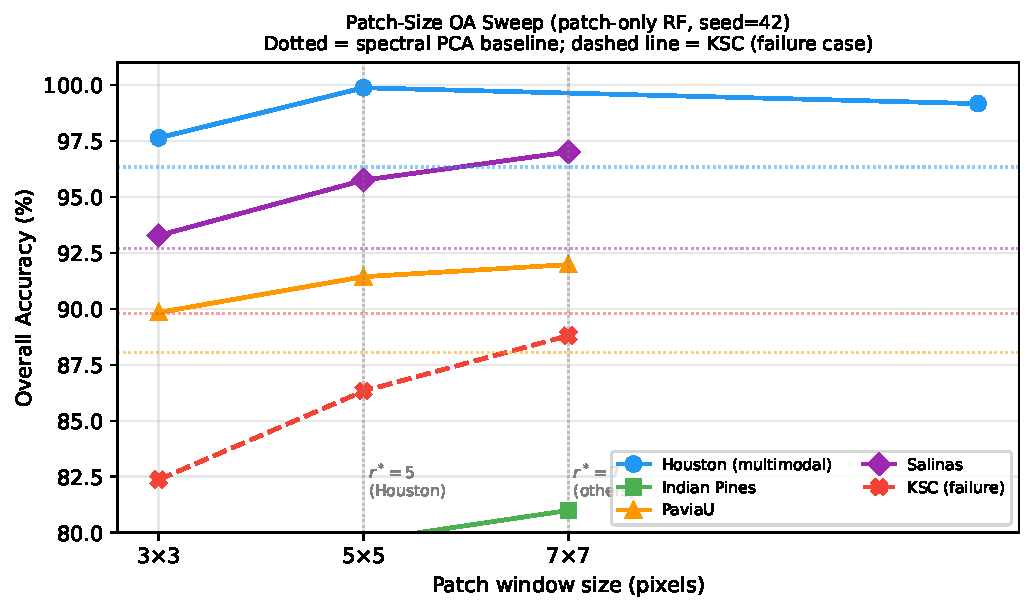
\includegraphics[width=0.48\textwidth]{fig1_patch_sweep.pdf}
  \hfill
  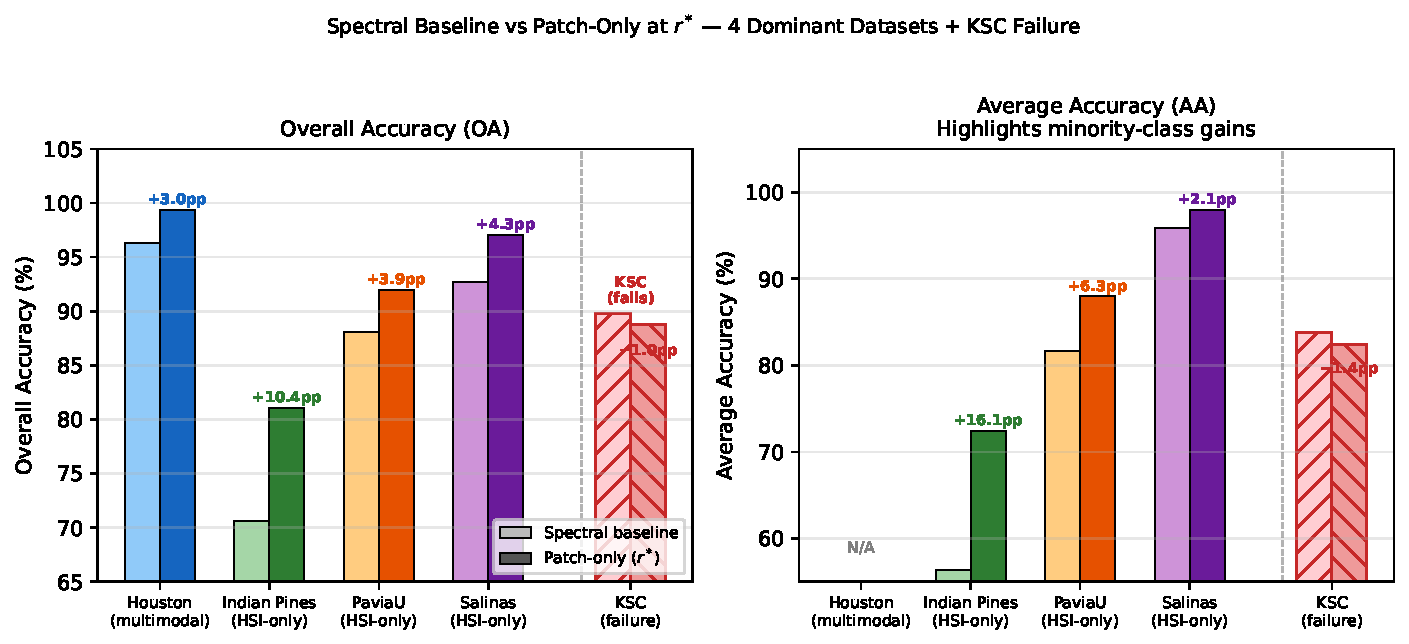
\includegraphics[width=0.48\textwidth]{fig2_oa_aa_comparison.pdf}
  \caption{%
    \textbf{Left (Fig.\,1):} Patch-size OA sweep across five datasets.
    Dashed lines indicate spectral PCA baselines.
    Performance saturates at scene-dependent $\rstar$
    ($5{\times}5$ Houston; $7{\times}7$ Indian Pines and PaviaU).
    \textbf{Right (Fig.\,2):} OA and AA comparison between spectral
    baseline and patch-only representation at $\rstar$.
    AA gains exceed OA gains on Indian Pines (minority rescue).%
  }
  \label{fig:sweep}
\end{figure*}

\begin{figure}[t]
  \centering
  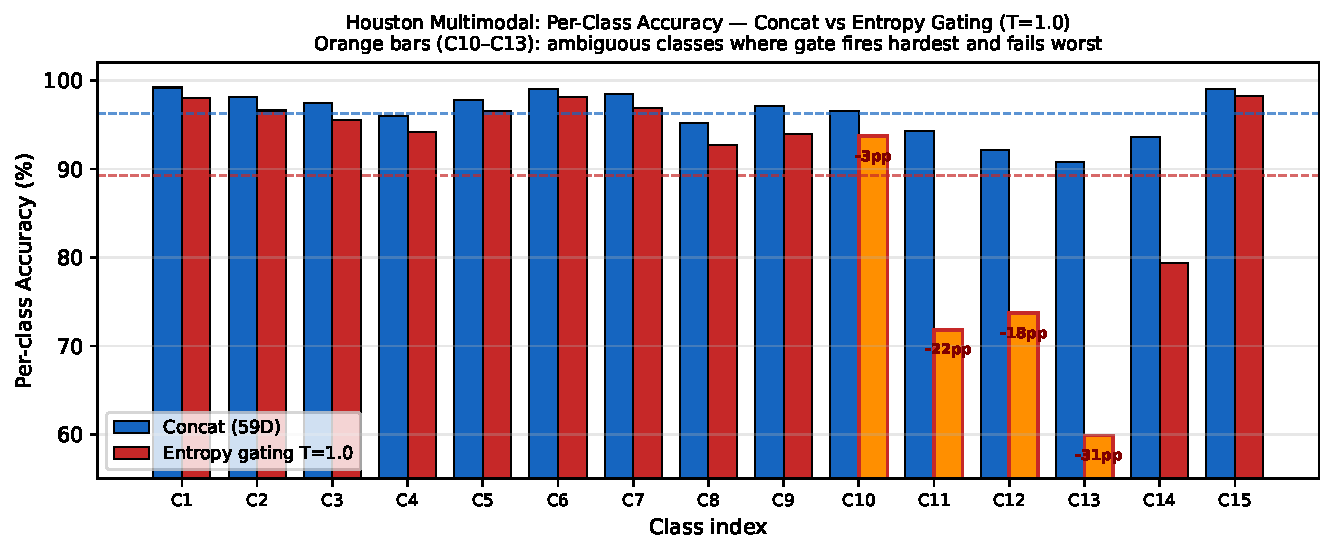
\includegraphics[width=\columnwidth]{fig3_gating_failure.pdf}
  \caption{%
    Houston per-class accuracy: concat baseline vs.\
    entropy gating ($T{=}1.0$). Classes C10--C13 (orange bars) are
    spectrally ambiguous; gate confidence is lowest there, causing
    14--31\pp\ accuracy decline. $\mathrm{corr}(\max w,
    \mathrm{correct}) \approx -0.08$ globally.%
  }
  \label{fig:gating}
\end{figure}

% ============================================================
\bibliographystyle{IEEEtran}
\bibliography{locality_dominance_refs}

\end{document}
